To showcase the implementation of the above schemes, numerical values were prescribed in Python code.
The numerical conditions are as follows:
\begin{equation}
	\label{eq:numerical-conditions}
	\begin{alignedat}{3}
		&\Delta t = 0.001 \qquad &&\frac{\Delta t}{\Delta x} = 0.2 \\
		&\nu = 10^{-2} \qquad &&L = 20 \quad \qquad T = 0.5 \\
		&u_L = 0.5 \qquad &&u_R = 1 \\
		&\alpha = -1 \qquad &&\beta = -1
	\end{alignedat}
\end{equation}
The quantity $\Delta t / \Delta x$ is known as the Courant--Friedrich--Lewy (CFL) number and is commonly seen in stability analyses of numerical methods.
It is generally introduced using a simple linear problem, such as:
\begin{equation}
	\label{eq:simple-cfl-ex}
	\pdv{u}{x}+a\pdv{u}{x}=0
\end{equation}
The CFL number for \cref{eq:simple-cfl-ex} would be $a\frac{\Delta t}{\Delta x}$ for a first-order explicit upwind scheme.\footnote{This just means a simple finite difference scheme.}~\autocite{caminhaCFLConditionHow2017}
For many schemes, a CFL number of less 1 is safe from instability while time-stepping.

With the above specifications, each computation began with the same initial condition (see \cref{fig:initial condition}).
For convenience, intermediate steps of $t=0.10$ (\cref{fig:0.1-figures}) and $t=0.25$ (\cref{fig:0.25-figures}) have been included along with the final time, $t=0.50$ (\cref{fig:final-figures}).
Additional solution sets can be created by running the code in the repository; however, only $\nu=10^{-2}$ is included in this report.
Additionally, the analytical solution adapted from~\autocite{cameronNOTESBURGERSEQUATION} for Dirichlet boundary conditions has been plotted as a proof of methods.\footnote{The solution given in~\autocite{cameronNOTESBURGERSEQUATION} is specified for an infinite domain. Because this is computationally impossible, the reader is urged to take the analytical solution plotted as an approximation.}
The solution is given as:
\begin{equation}
	\label{eq:analytical-burgers-solution}
	u(x,t)=\frac{u_R+u_L}{2}-\frac{u_L-u_R}{2}\tanh\left( \frac{\left( x_0-x-st\right)\left( u_L-u_R\right)    }{4\nu} \right)
\end{equation}
where the shock speed, $s$, is defined as:
\begin{equation}
	\label{eq:shock-speed}
	\begin{split}
		s&=\frac{f(u_L)-f(u_R)}{u_L-u_R}\\
		&=\left( \frac{u_L^2}{2}-\frac{u_R^2}{2} \right)/\left( u_L-u_R \right)\\
		&=\frac{u_L+u_R}{2}
	\end{split}
\end{equation}
Variables $u_L$ and $u_R$ are defined as in the initial conditions (\cref{eq:initial-condition}) and $x_0=10$.
Analytical solutions for Neumann and periodic boundary conditions are not included in this report, so \cref{eq:analytical-burgers-solution,eq:shock-speed} are only found in the Dirichlet code.
\begin{figure}
	\centering
	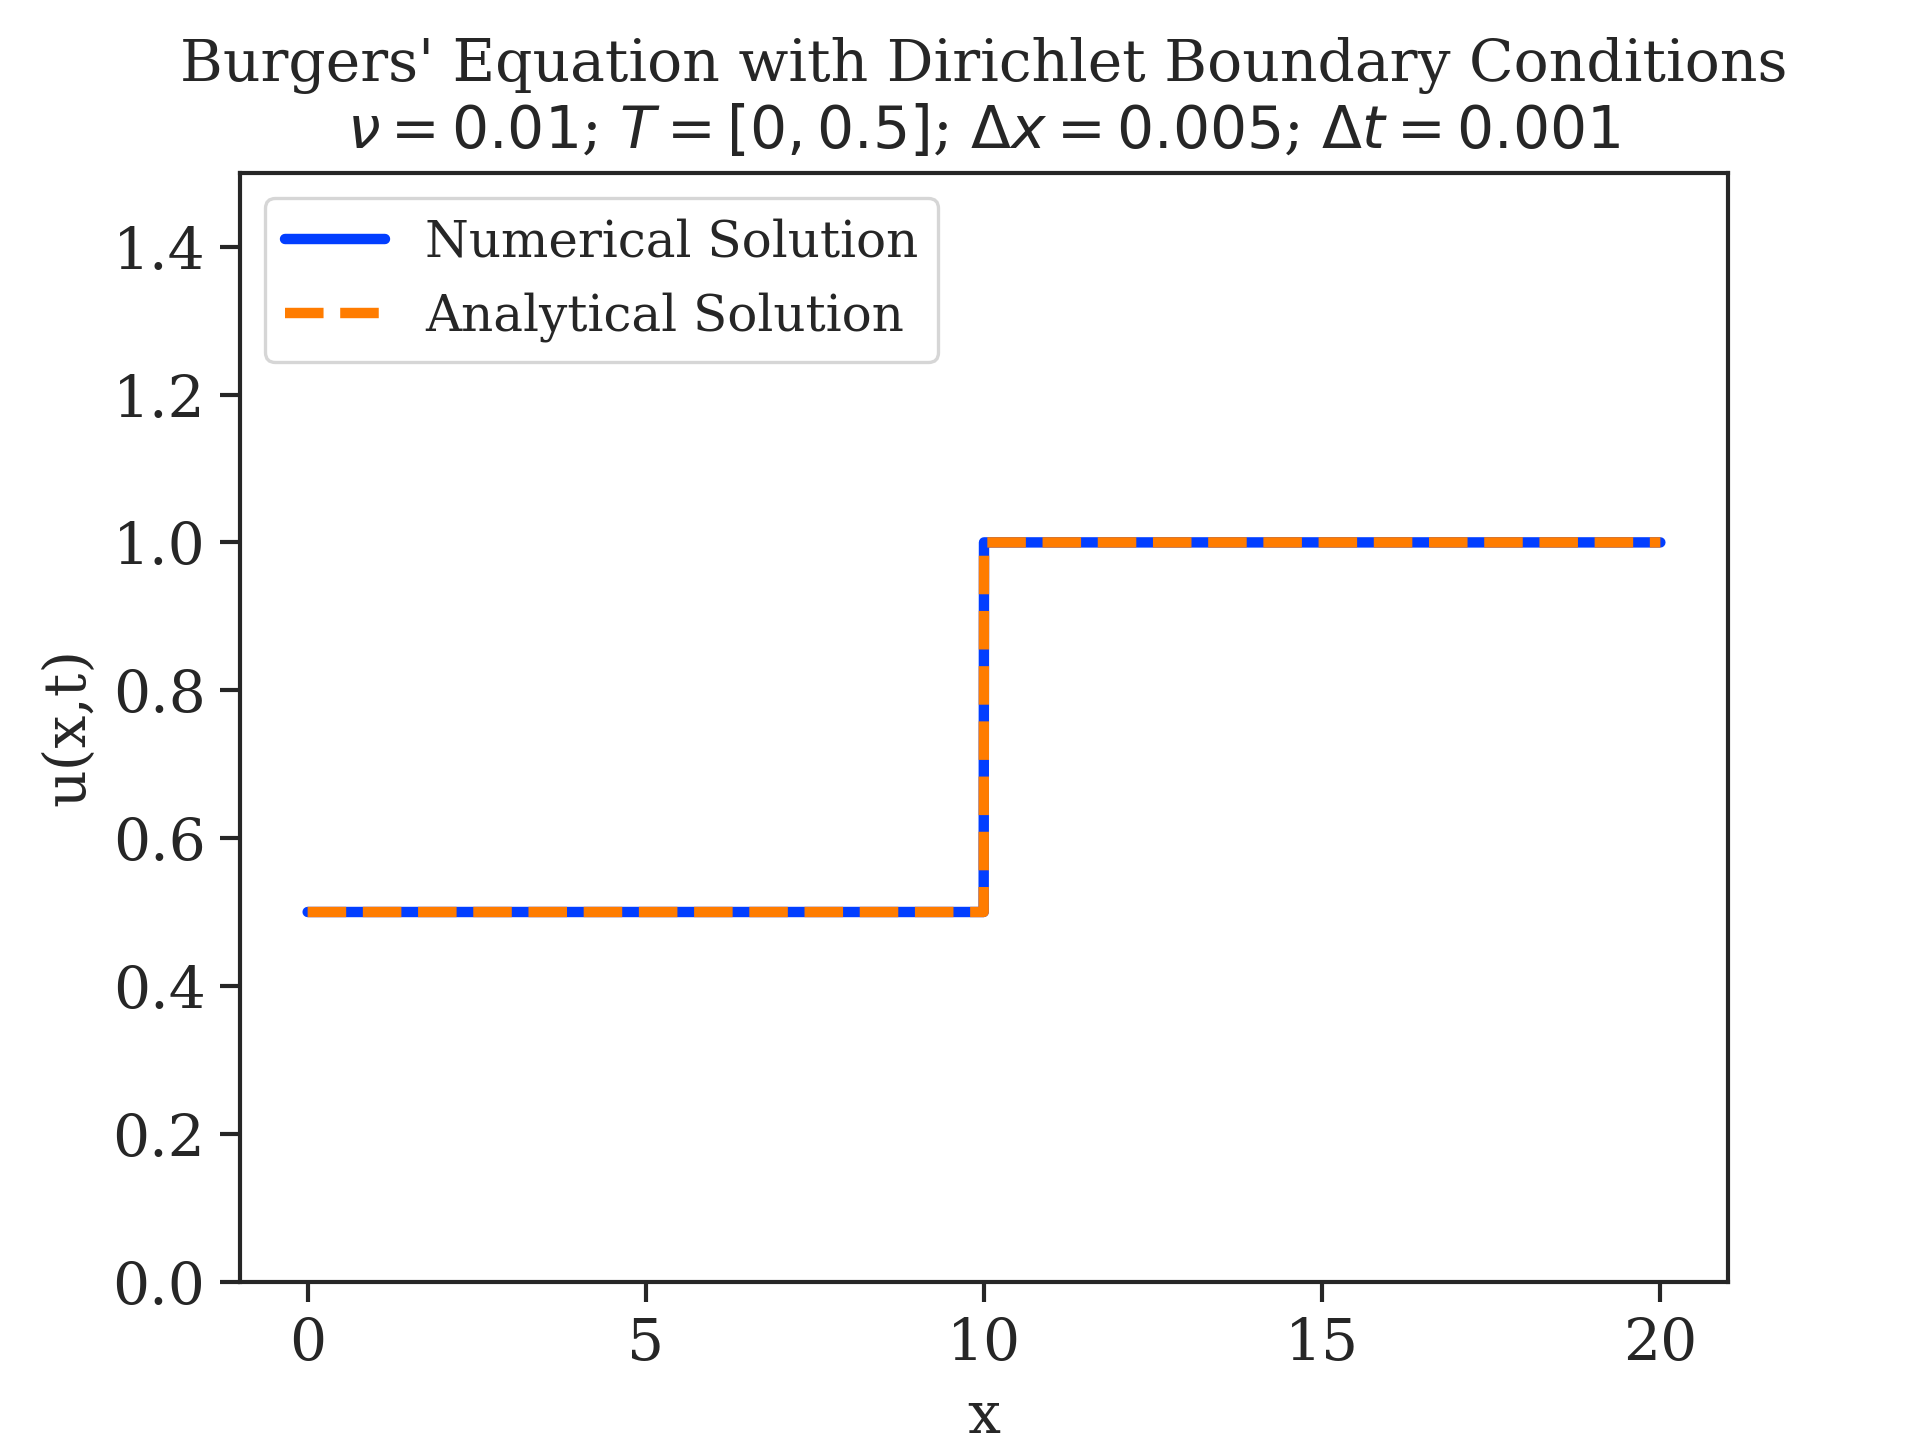
\includegraphics[width=0.8\textwidth]{../dirichlet_BC/images_nu=0.01/0_plot}
	\caption{Implemented Initial Condition}
	\label{fig:initial condition}
\end{figure}

\begin{figure}
	\centering
	\begin{subfigure}{0.55\linewidth}
		\centering
		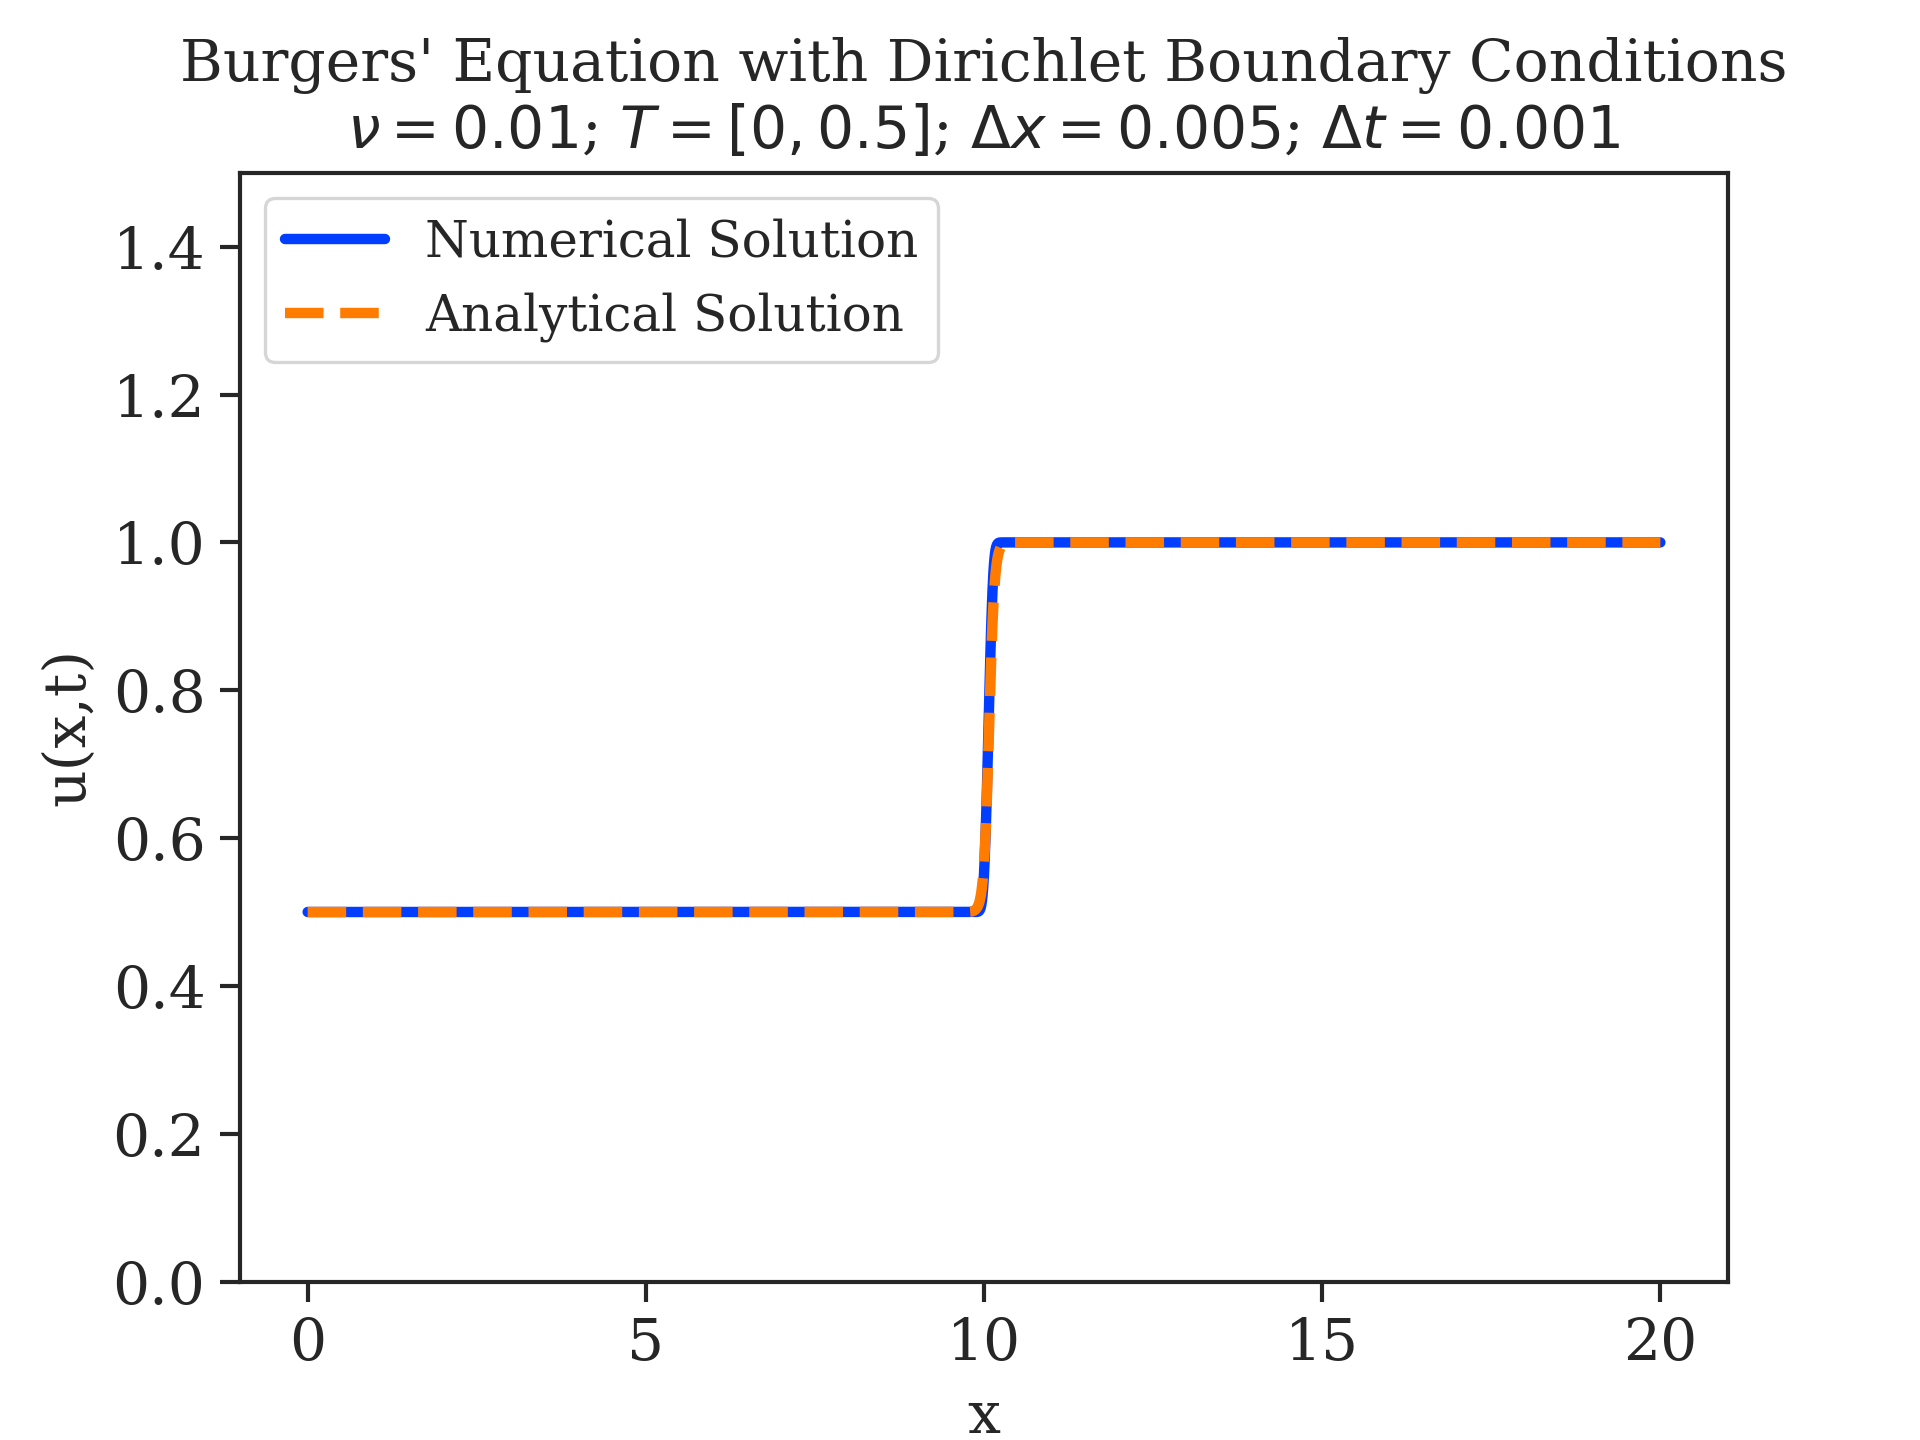
\includegraphics[width=\linewidth]{../dirichlet_BC/images_nu=0.01/100_plot}
		\caption{Inhomogeneous Dirichlet}
	\end{subfigure}
	\hfill
	\begin{subfigure}{0.55\linewidth}
		\centering
		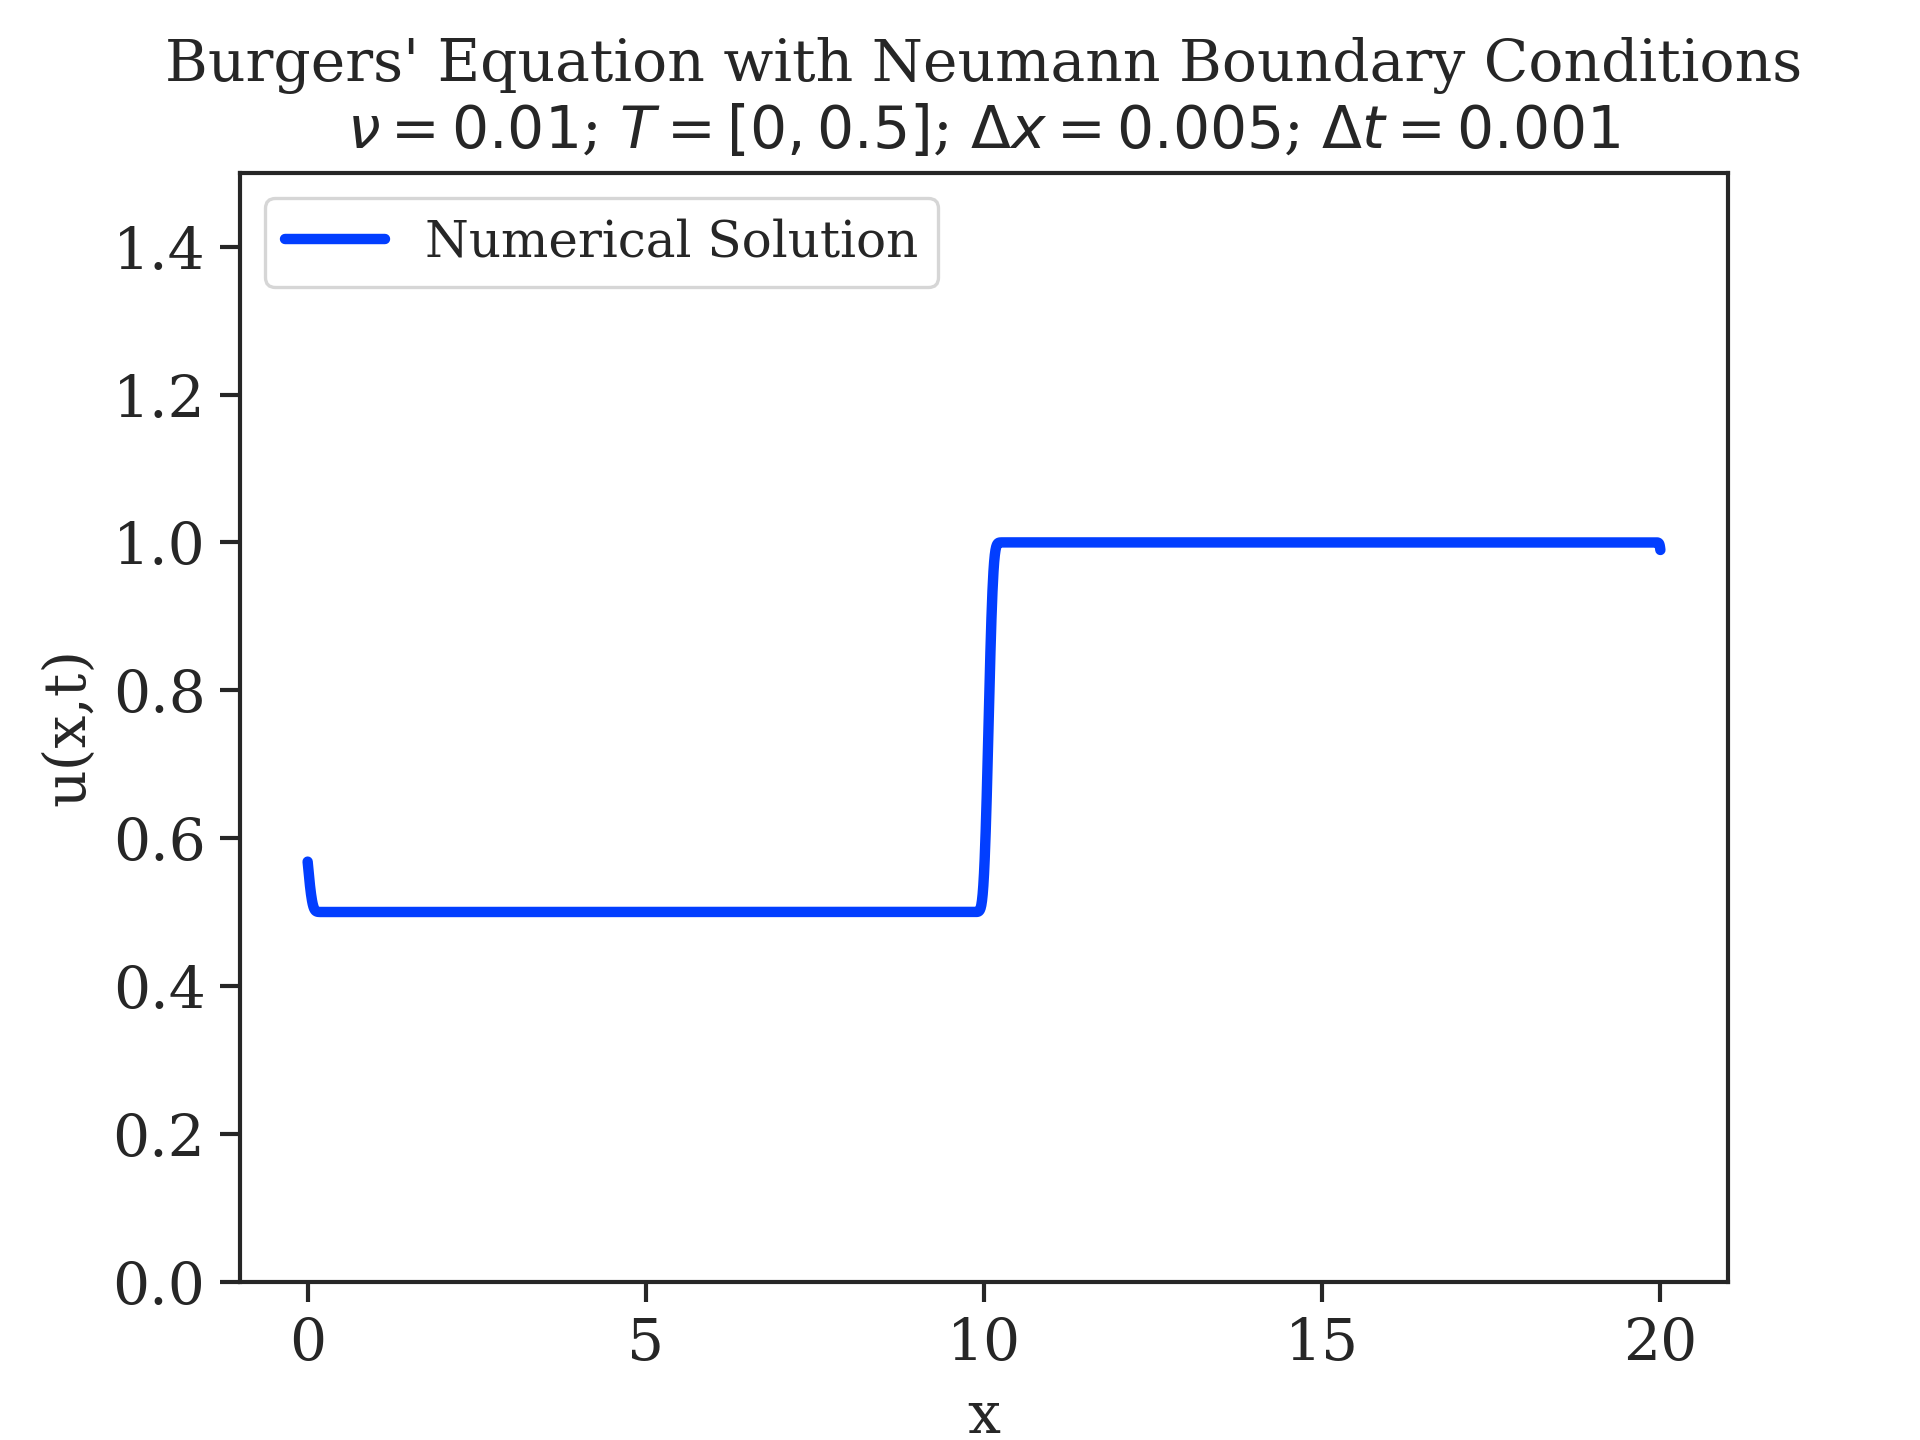
\includegraphics[width=\linewidth]{../neumann_BC/images_nu=0.01/100_plot}
		\caption{Inhomogeneous Neumann}
	\end{subfigure}
	\hfill
	\begin{subfigure}{0.55\linewidth}
		\centering
		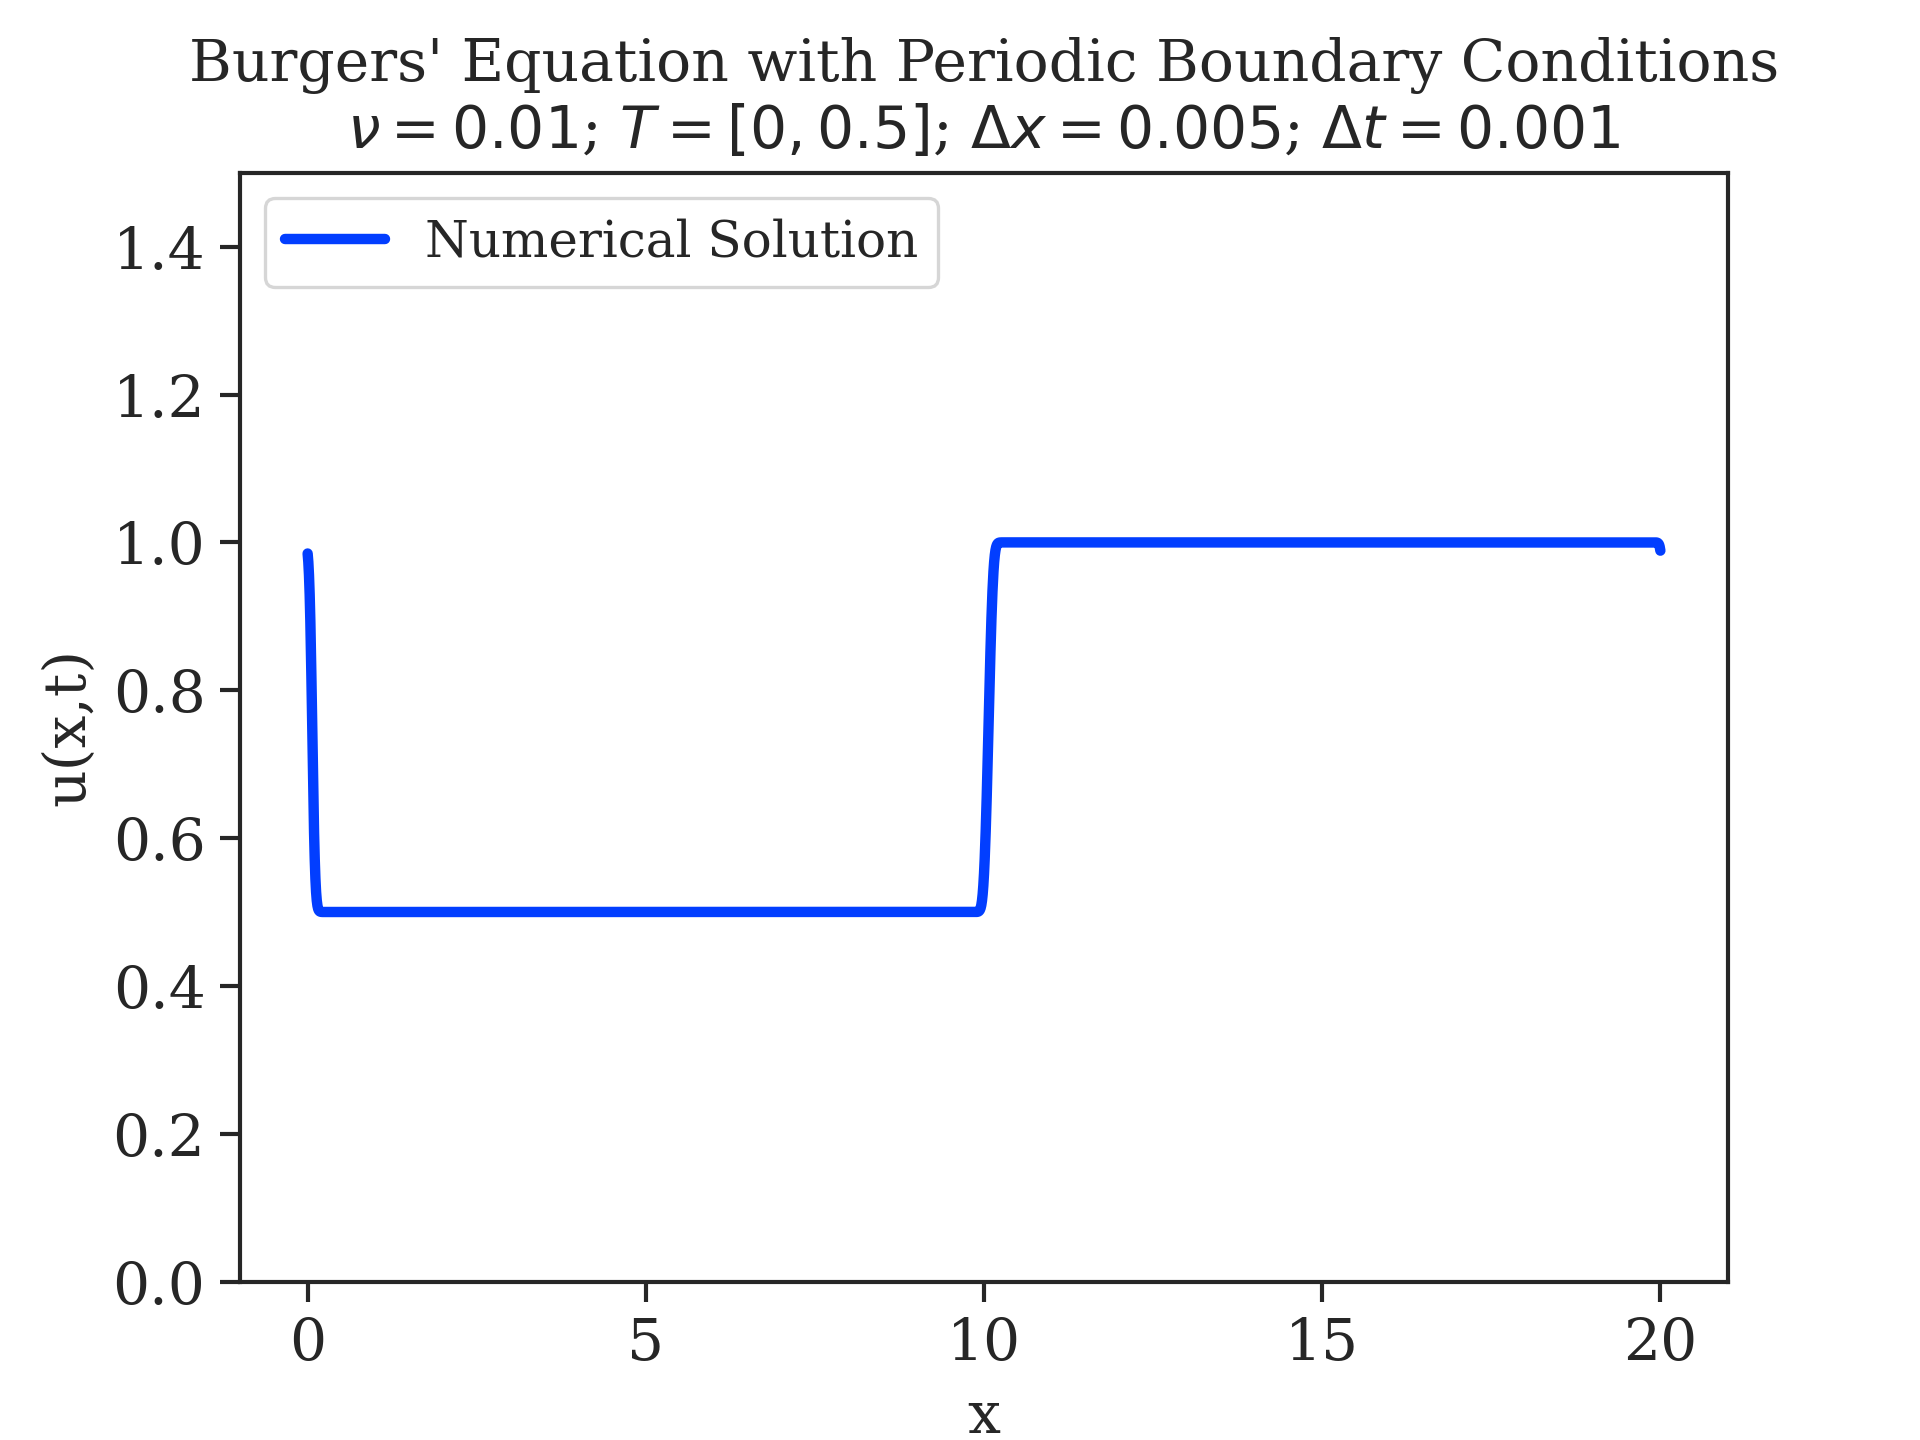
\includegraphics[width=\linewidth]{../periodic_BC/images_nu=0.01/100_plot}
		\caption{Periodic}
	\end{subfigure}

	\caption{Implemented Conditions $t=0.10$}
	\label{fig:0.1-figures}
\end{figure}

\begin{figure}
	\centering
	\begin{subfigure}{0.55\linewidth}
		\centering
		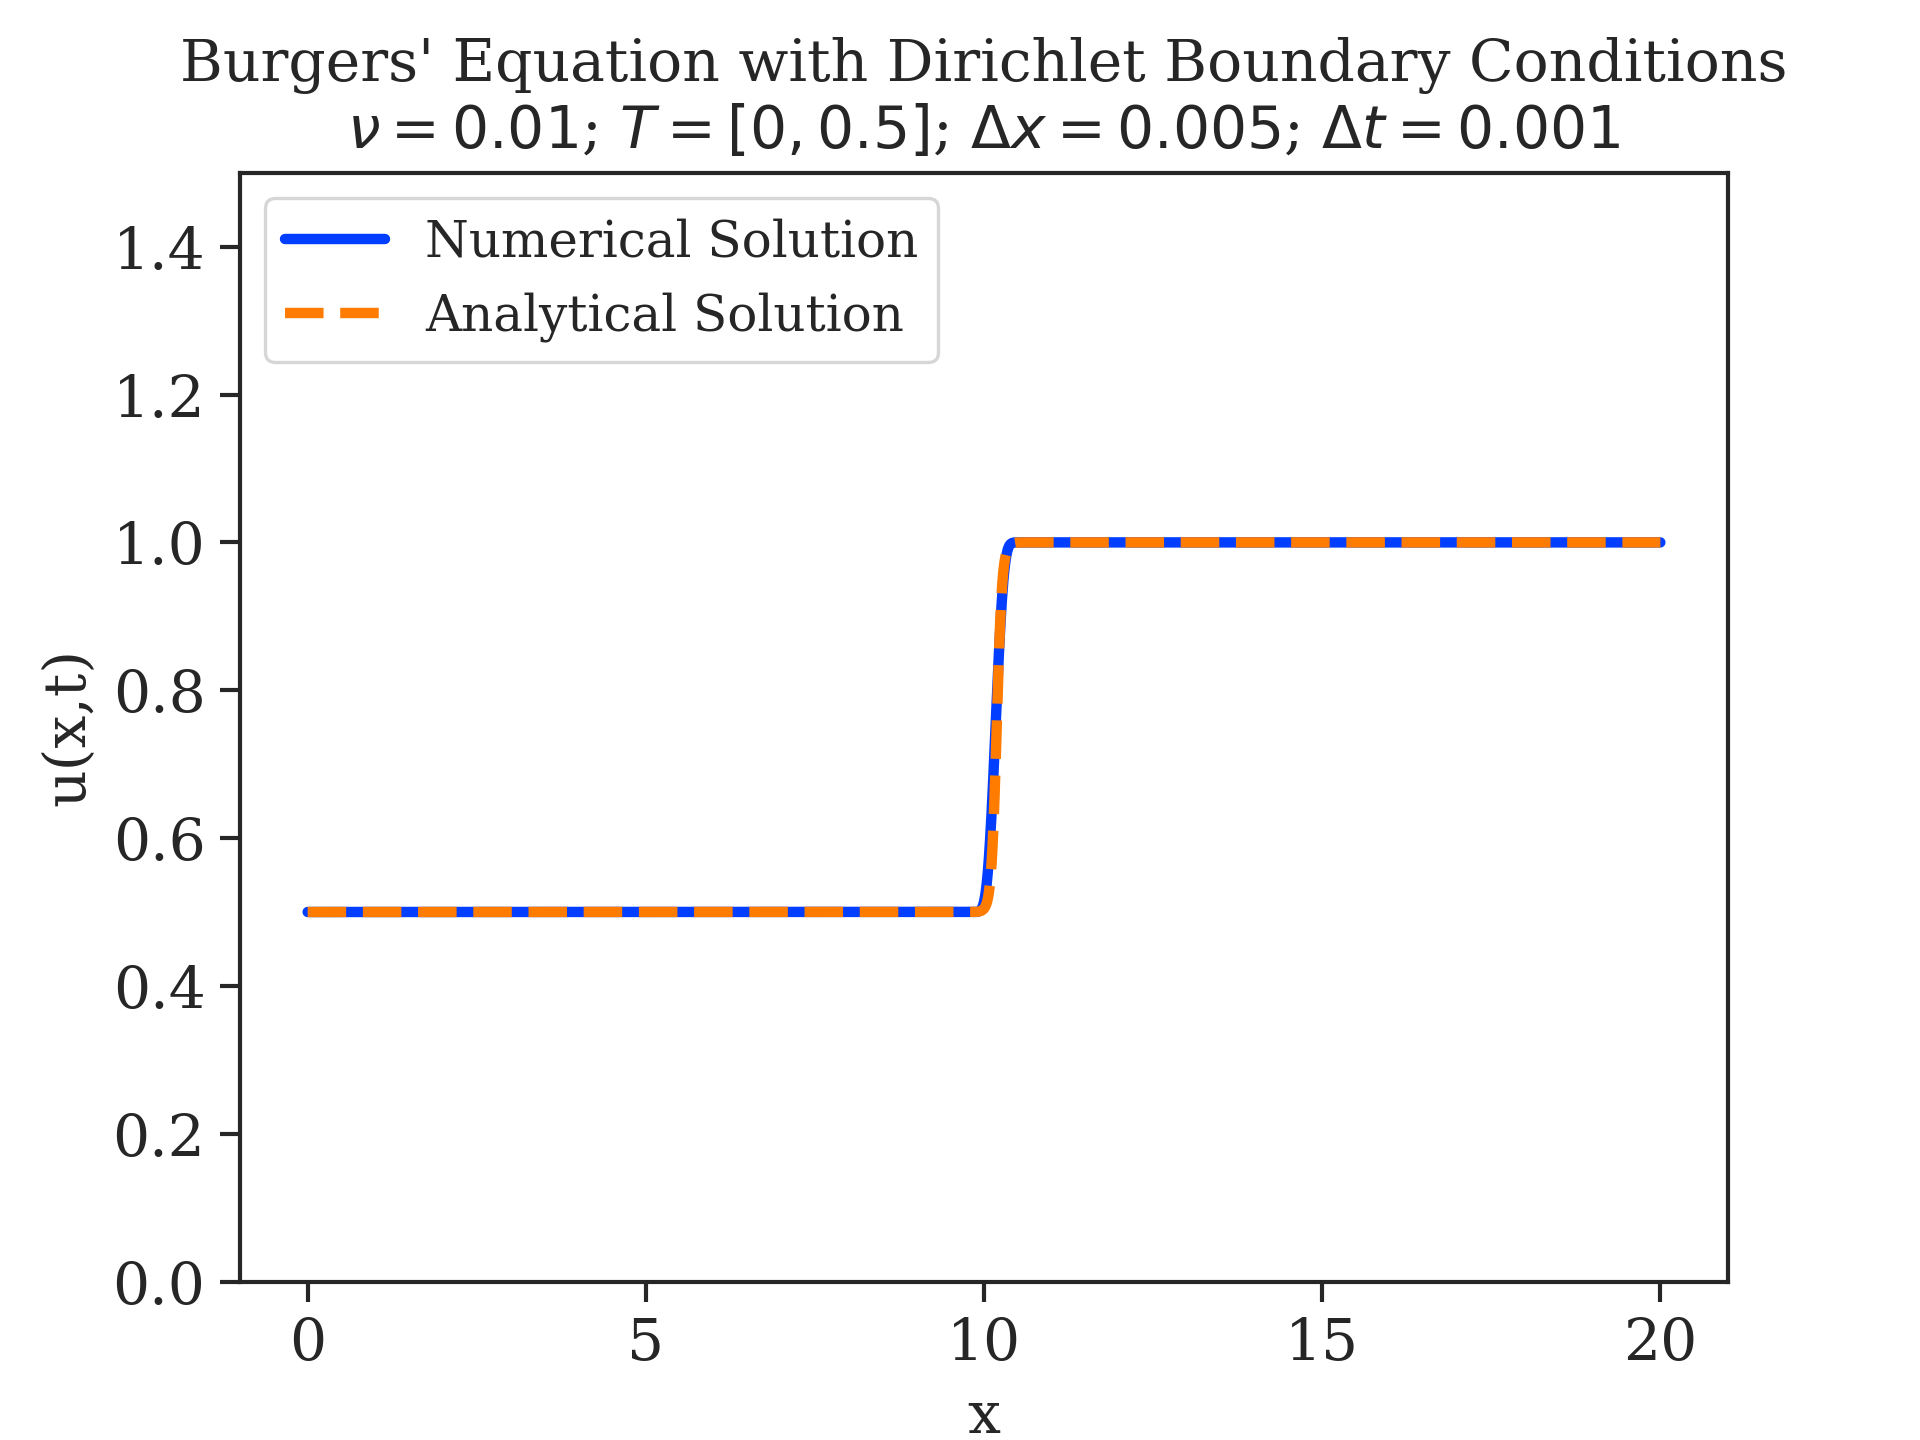
\includegraphics[width=\linewidth]{../dirichlet_BC/images_nu=0.01/250_plot}
		\caption{Inhomogeneous Dirichlet}
	\end{subfigure}
	\hfill
	\begin{subfigure}{0.55\linewidth}
		\centering
		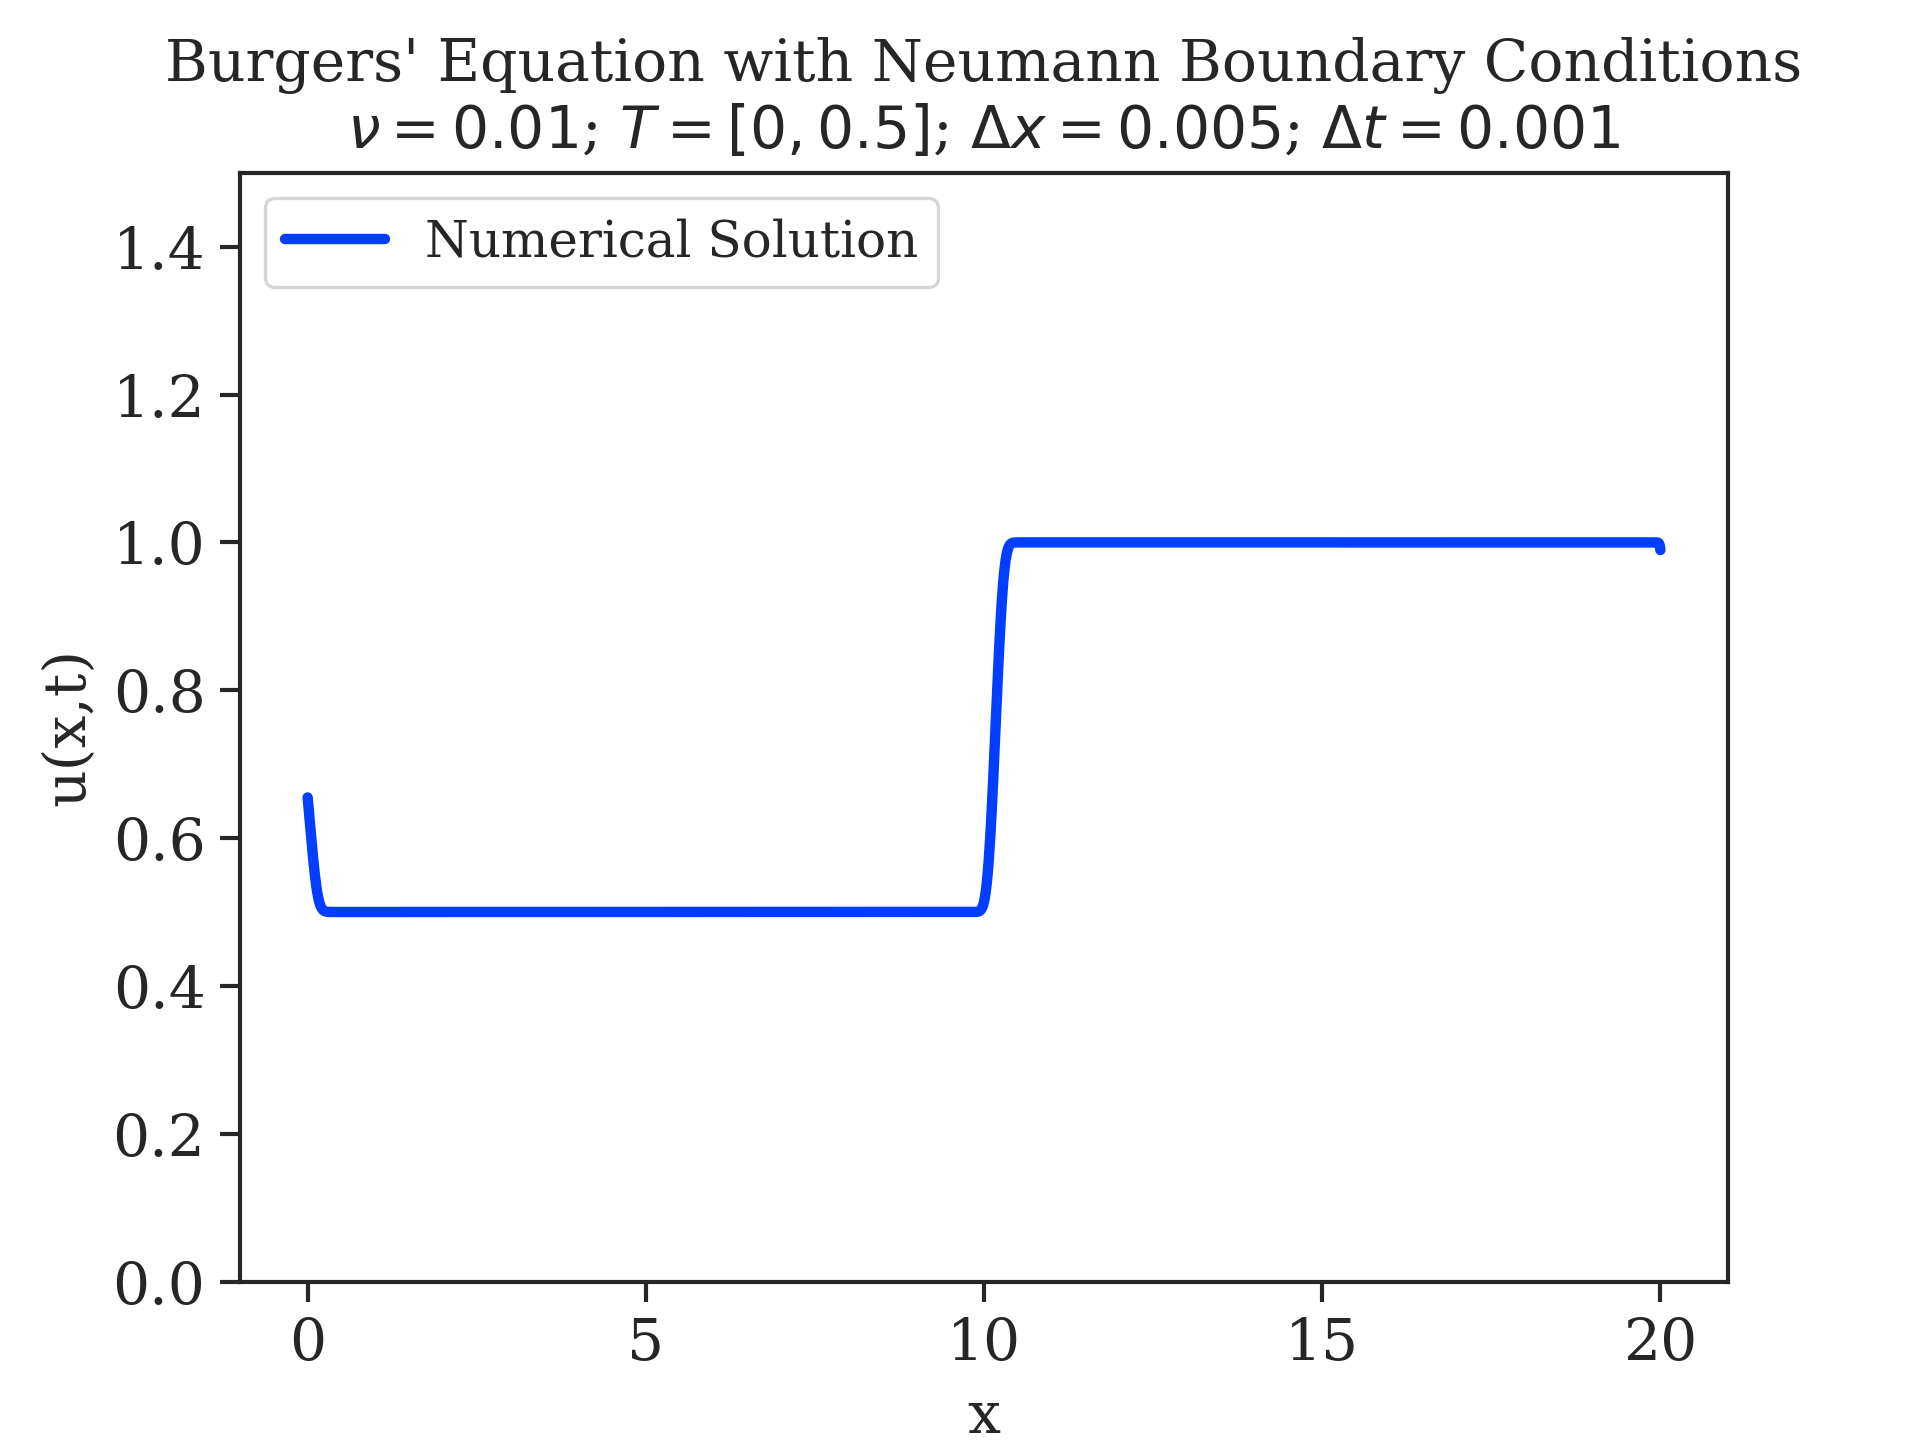
\includegraphics[width=\linewidth]{../neumann_BC/images_nu=0.01/250_plot}
		\caption{Inhomogeneous Neumann}
	\end{subfigure}
	\hfill
	\begin{subfigure}{0.55\linewidth}
		\centering
		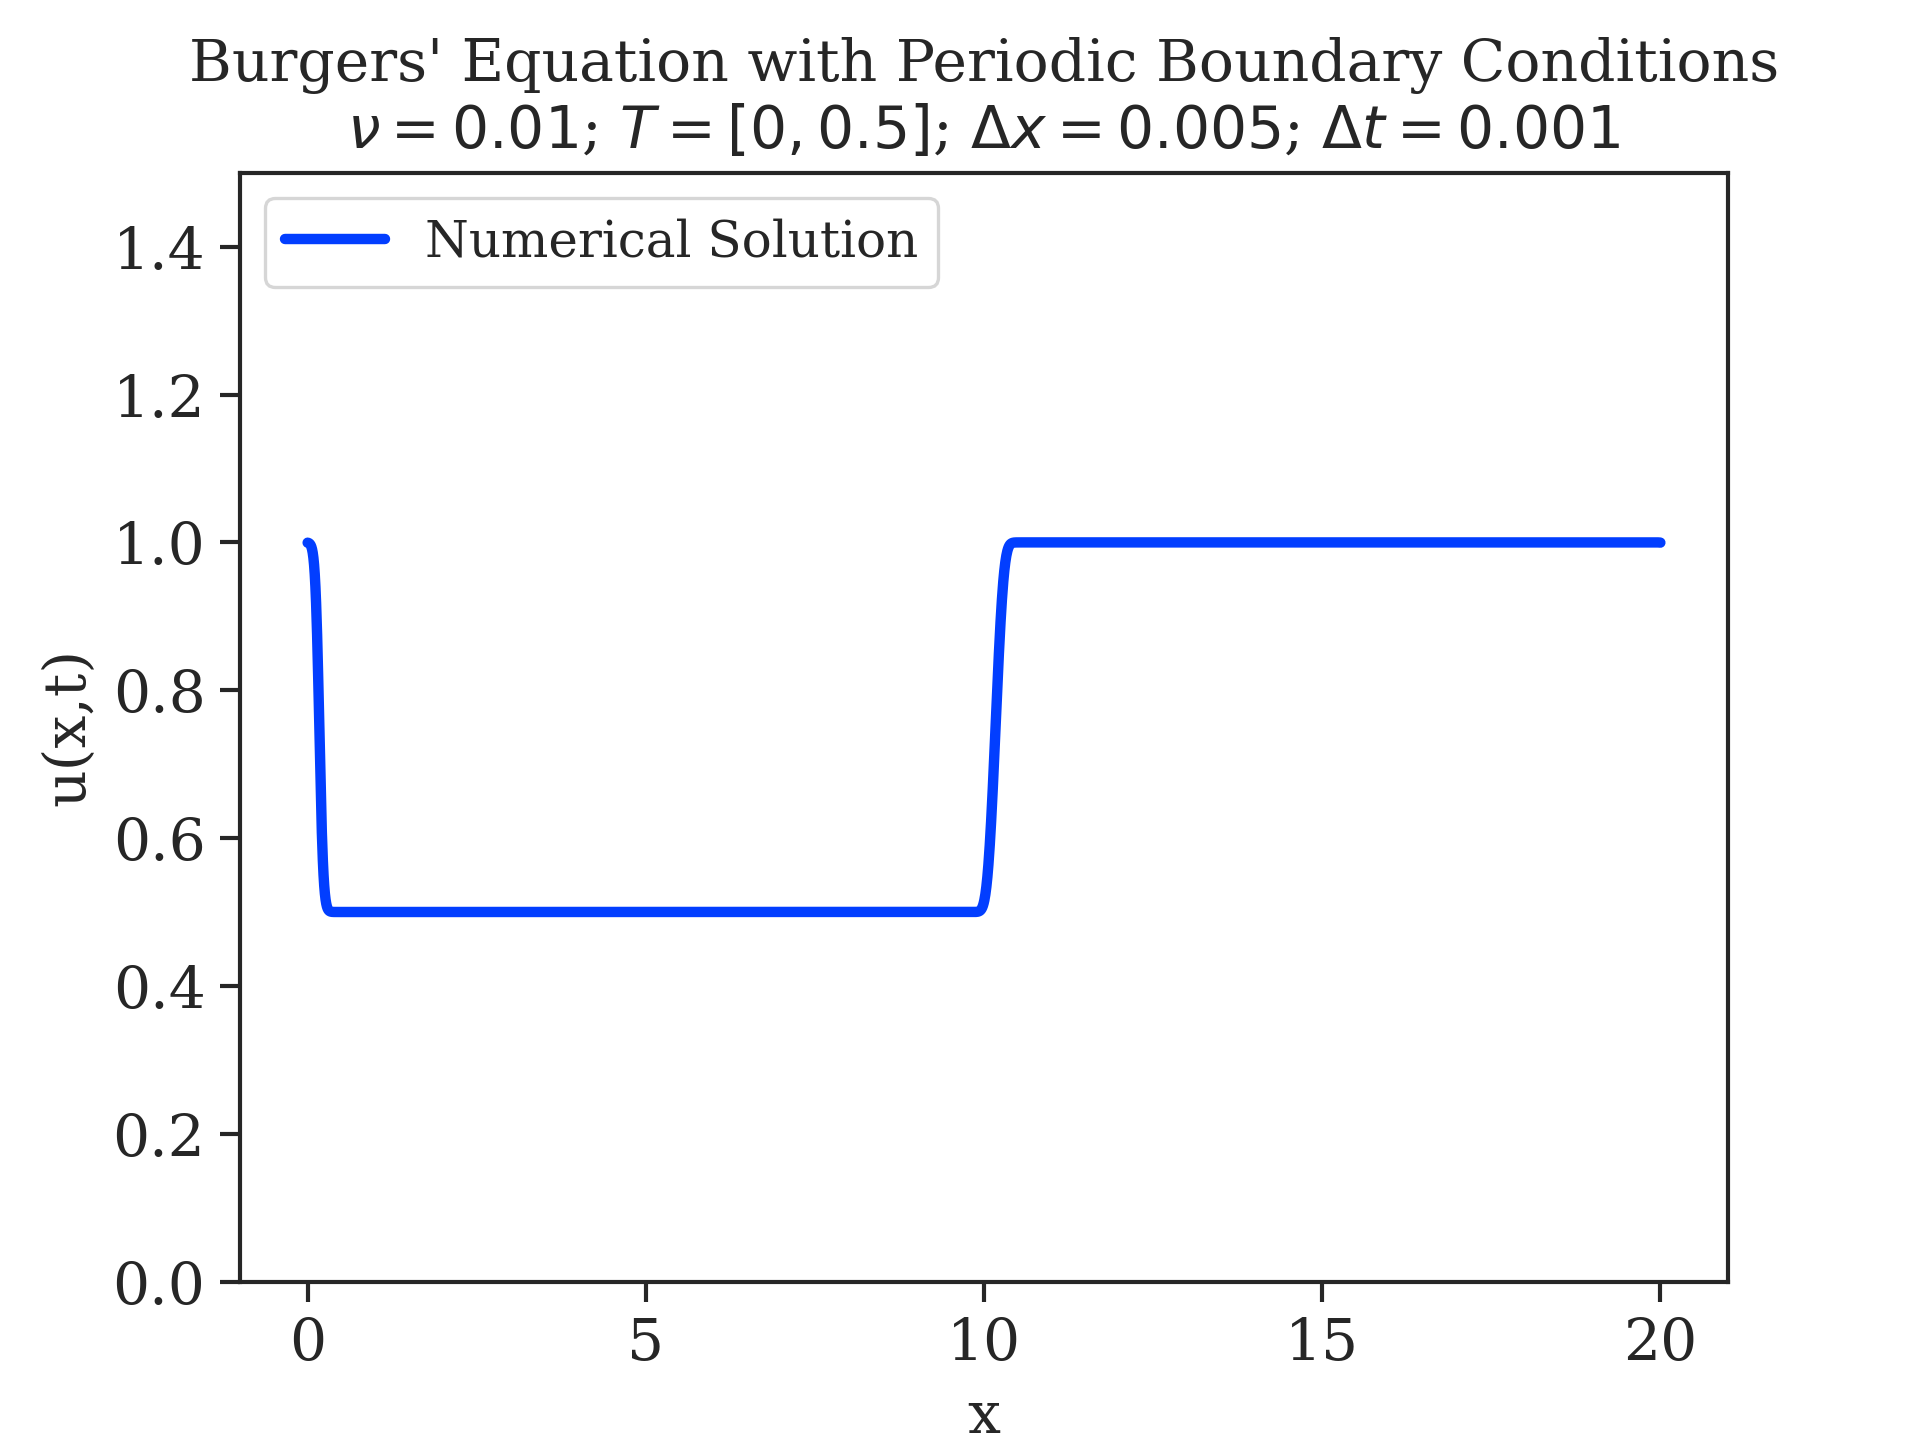
\includegraphics[width=\linewidth]{../periodic_BC/images_nu=0.01/250_plot}
		\caption{Periodic}
	\end{subfigure}

	\caption{Implemented Conditions $t=0.25$}
	\label{fig:0.25-figures}
\end{figure}

\begin{figure}
	\centering
	\begin{subfigure}{0.55\linewidth}
		\centering
		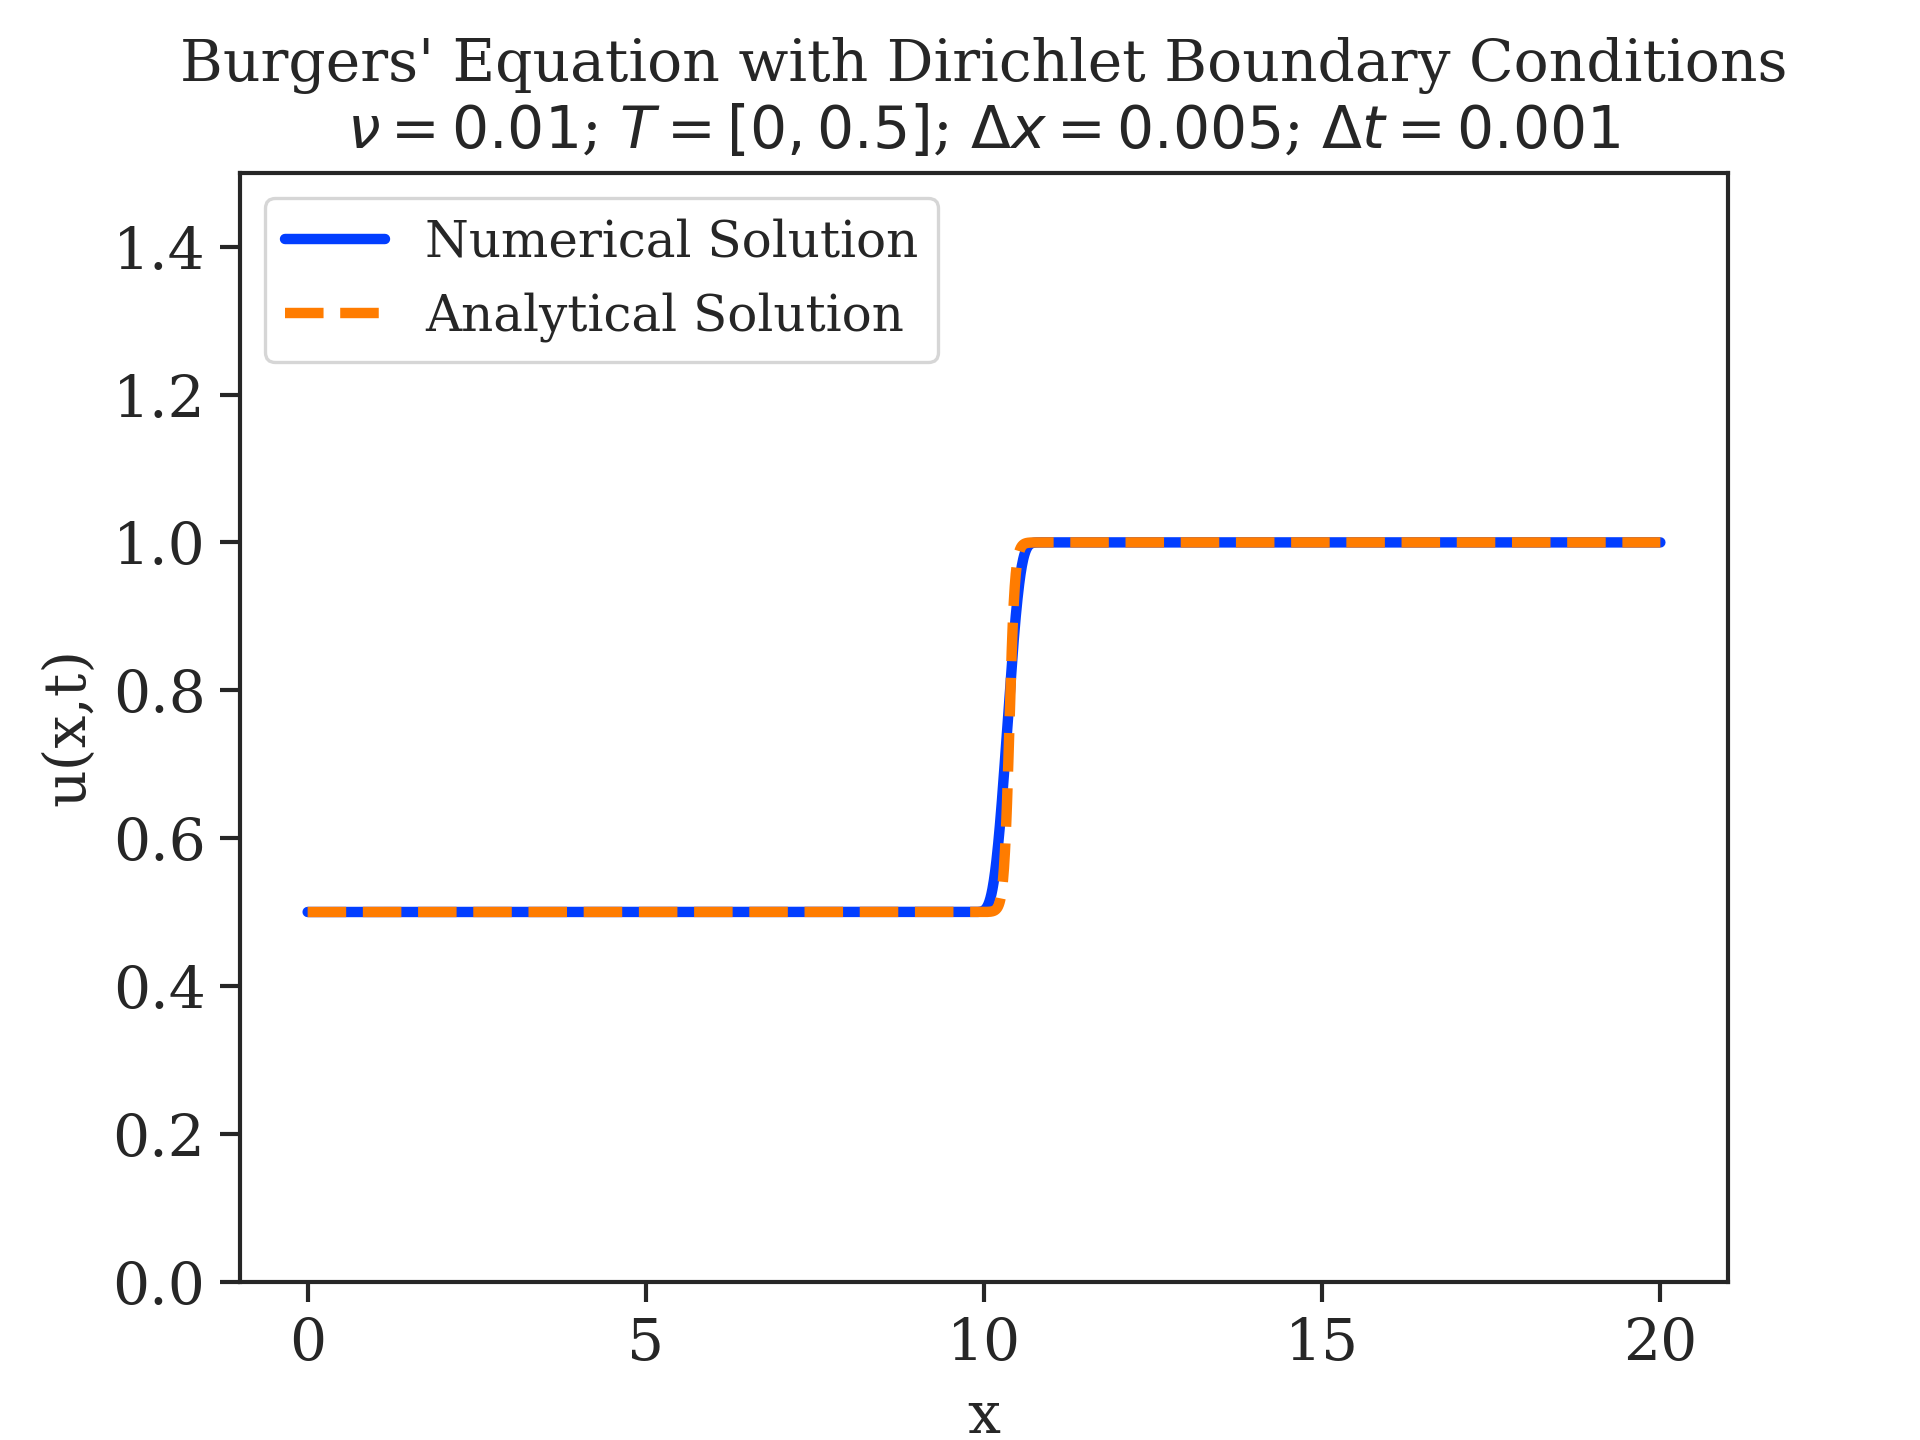
\includegraphics[width=\linewidth]{../dirichlet_BC/images_nu=0.01/500_plot}
		\caption{Inhomogeneous Dirichlet}
	\end{subfigure}
	\hfill
	\begin{subfigure}{0.55\linewidth}
		\centering
		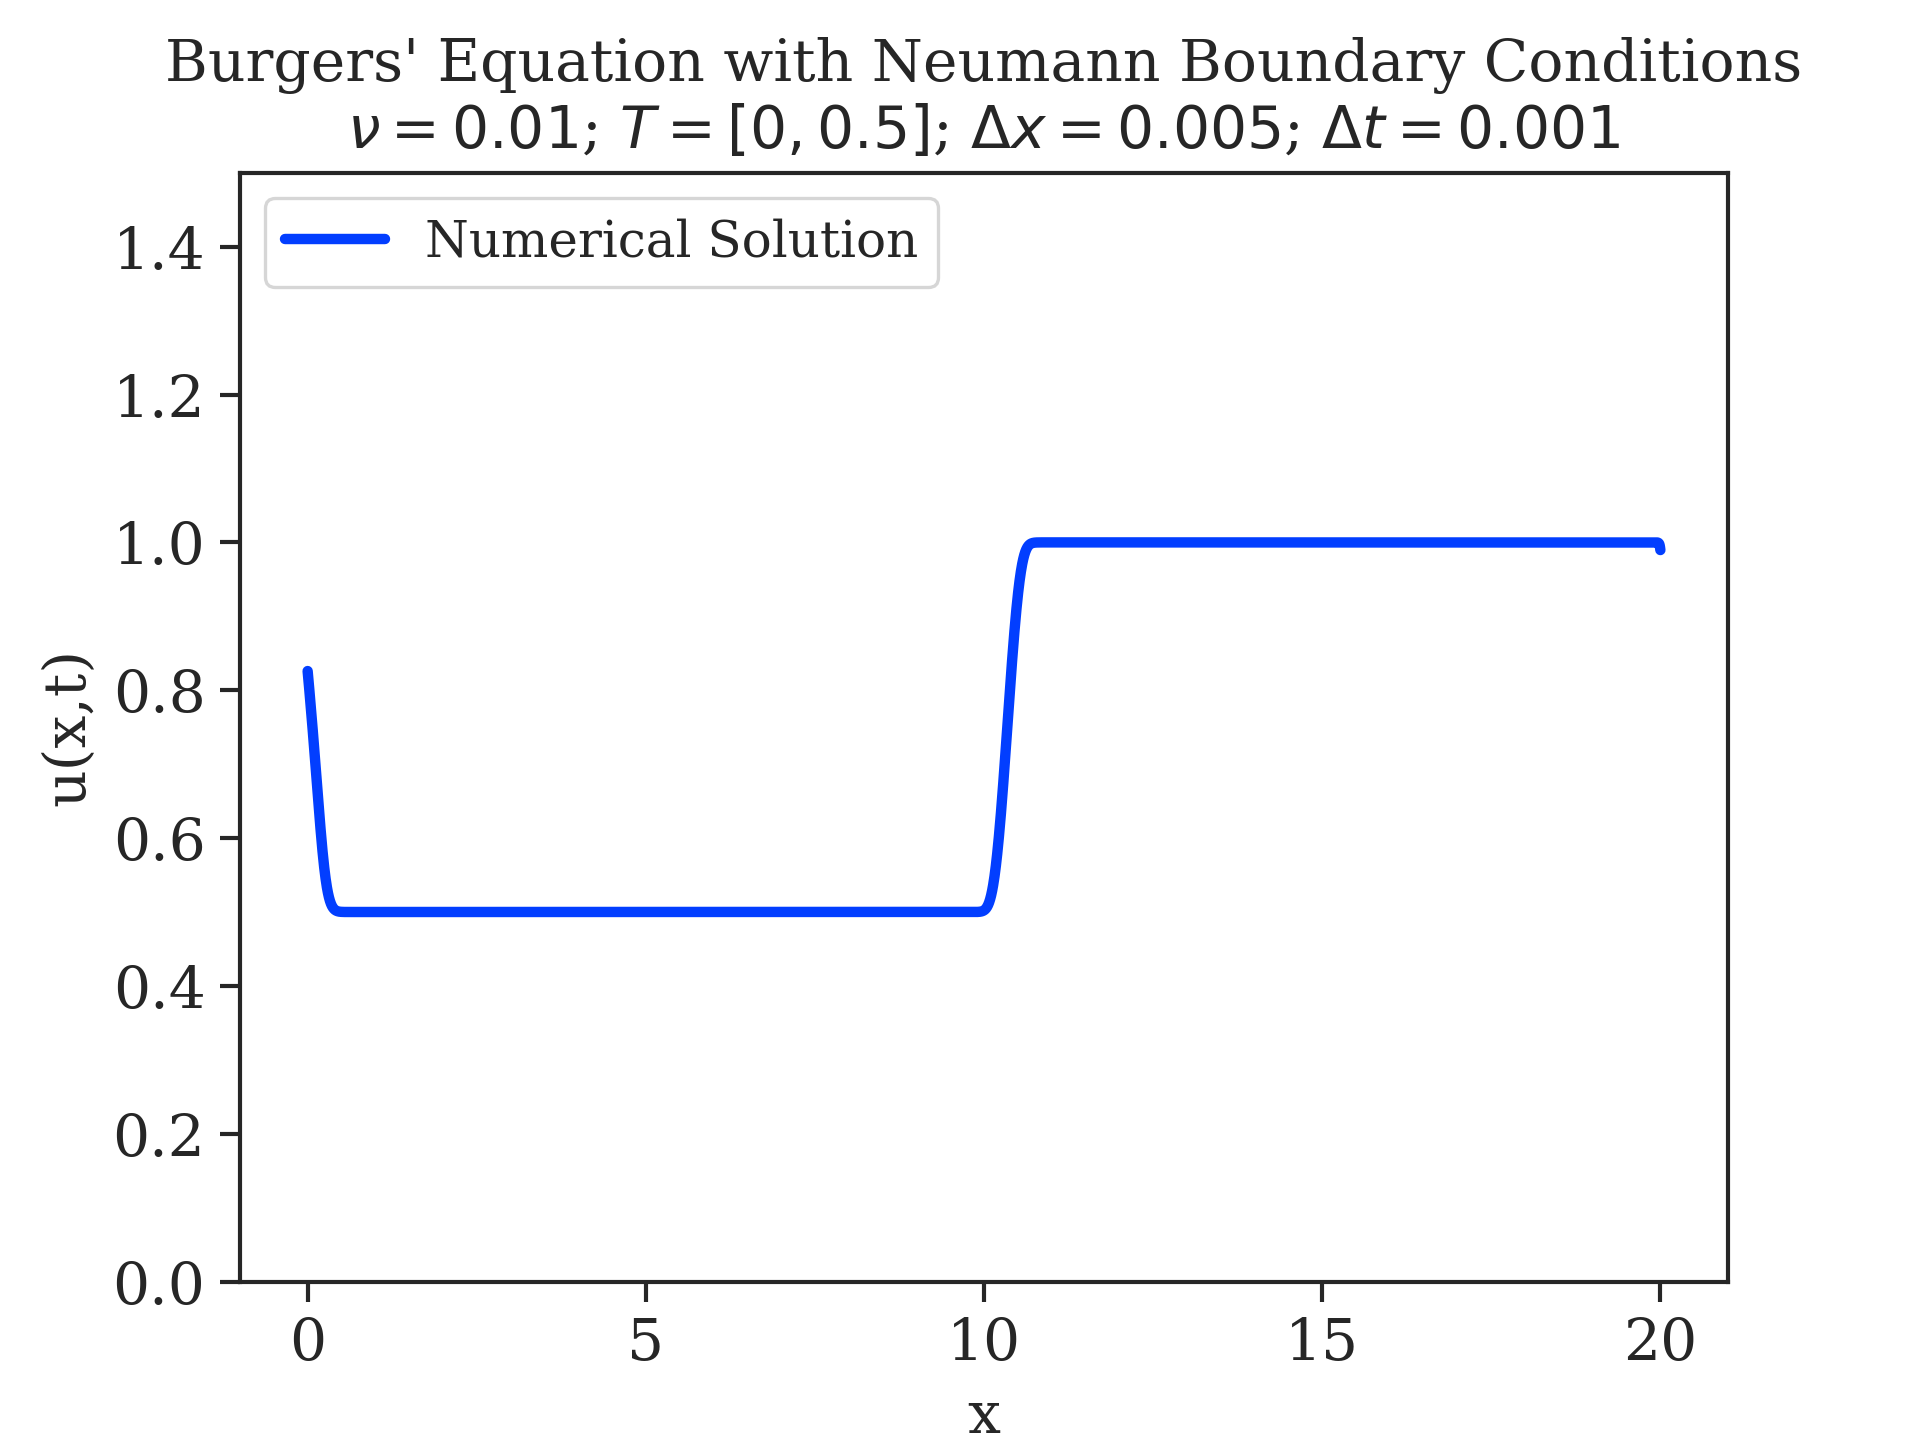
\includegraphics[width=\linewidth]{../neumann_BC/images_nu=0.01/500_plot}
		\caption{Inhomogeneous Neumann}
	\end{subfigure}
	\hfill
	\begin{subfigure}{0.55\linewidth}
		\centering
		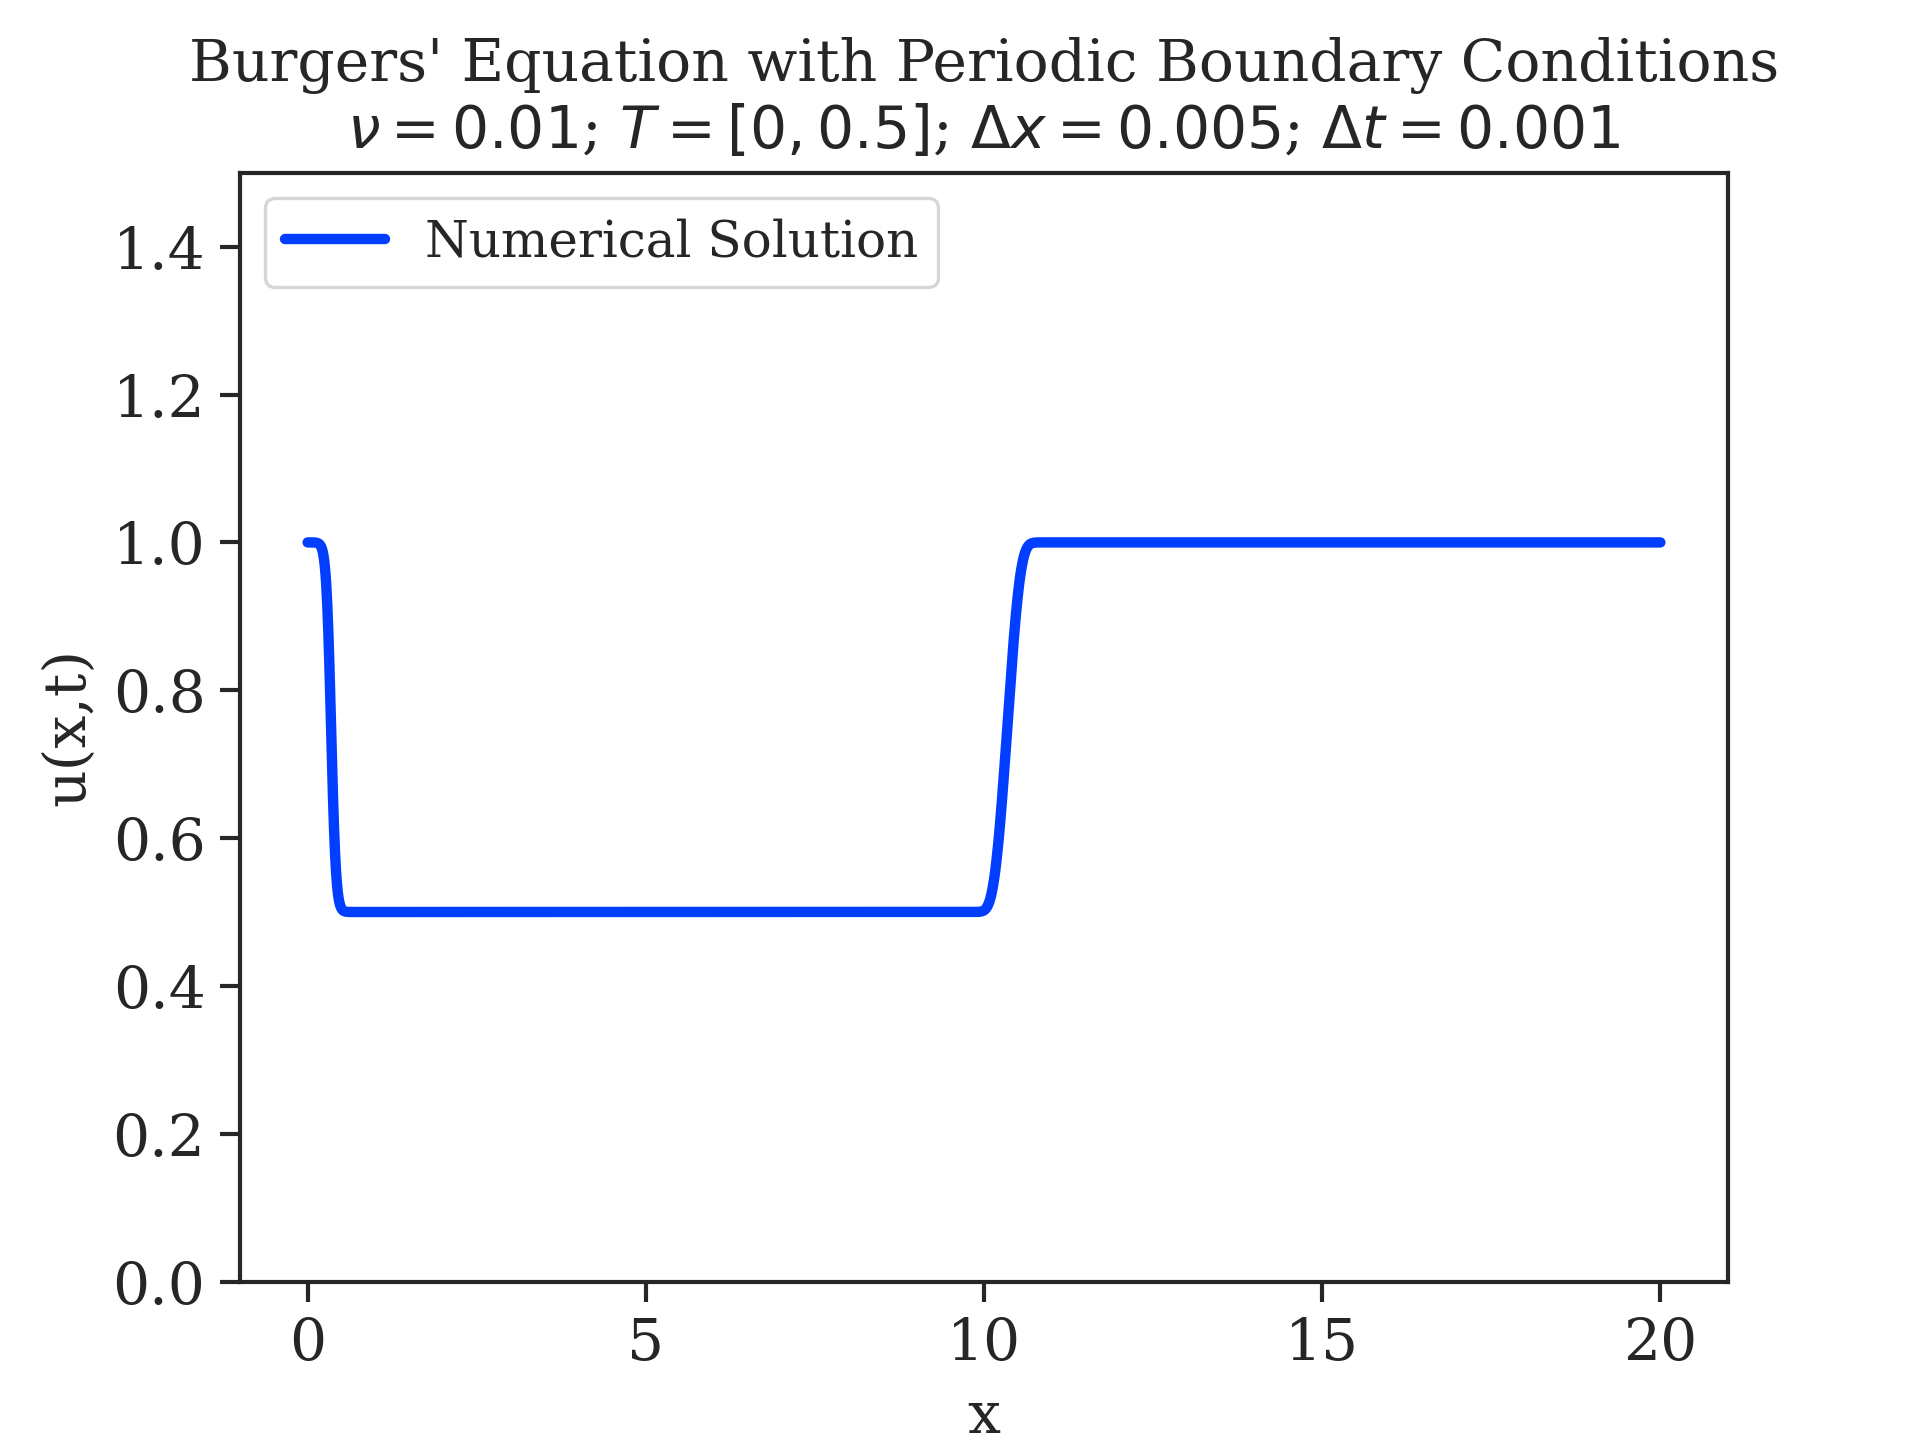
\includegraphics[width=\linewidth]{../periodic_BC/images_nu=0.01/500_plot}
		\caption{Periodic}
	\end{subfigure}
	\hfill

	\caption{Implemented Conditions $t=0.50$}
	\label{fig:final-figures}
\end{figure}

As mentioned in \cref{sec:problem-statement}, Burgers' equation was developed to study shocks and rarefactions in fluids, which that occur due to the nonlinear advective term present in the Navier-Stokes equations.
Because this paper's focus was on numerical methods and implementation, a mathematical analysis of these phenomena are not included.
For more studies on shocks and Burgers' equation, the author recommends~\autocite{salihBurgersEquation2016,cameronNOTESBURGERSEQUATION} among other resources.